\documentclass{article}

\usepackage{tikz} 
\usetikzlibrary{automata, positioning, arrows} 

\usepackage{amsthm}
\usepackage{amsfonts}
\usepackage{amsmath}
\usepackage{amssymb}
\usepackage{tikz}
\usepackage{fullpage}
\usepackage{color}
\usepackage{parskip}
\usepackage{hyperref}
  \hypersetup{
    colorlinks = true,
    urlcolor = blue,       % color of external links using \href
    linkcolor= blue,       % color of internal links 
    citecolor= blue,       % color of links to bibliography
    filecolor= blue,        % color of file links
    }
    
\usepackage{listings}
\usepackage[utf8]{inputenc}                                                    
\usepackage[T1]{fontenc}                                                       

\definecolor{dkgreen}{rgb}{0,0.6,0}
\definecolor{gray}{rgb}{0.5,0.5,0.5}
\definecolor{mauve}{rgb}{0.58,0,0.82}

\lstset{frame=tb,
  language=haskell,
  aboveskip=3mm,
  belowskip=3mm,
  showstringspaces=false,
  columns=flexible,
  basicstyle={\small\ttfamily},
  numbers=none,
  numberstyle=\tiny\color{gray},
  keywordstyle=\color{blue},
  commentstyle=\color{dkgreen},
  stringstyle=\color{mauve},
  breaklines=true,
  breakatwhitespace=true,
  tabsize=3
}

\theoremstyle{plain} 
   \newtheorem{theorem}{Theorem}[section]
   \newtheorem{corollary}[theorem]{Corollary}
   \newtheorem{lemma}[theorem]{Lemma}
   \newtheorem{proposition}[theorem]{Proposition}
\theoremstyle{definition}
   \newtheorem{definition}[theorem]{Definition}
   \newtheorem{example}[theorem]{Example}
\theoremstyle{remark}    
  \newtheorem{remark}[theorem]{Remark}

\title{CPSC-354 Report}
\author{Zach Pratto  \\ Chapman University}

\date{\today} 

\begin{document}

\maketitle

\begin{abstract}
This is the place to write an abstract. Not much has been abstracted yet.
\end{abstract}

\setcounter{tocdepth}{3}
\tableofcontents

\section{Introduction}\label{intro}

\section{Week by Week}\label{homework}

\subsection{Week 1}

Week 1 aligns with the first week of the semester. 

\subsubsection{Notes and Exploration}

This section is optional. 

\subsubsection{Homework}

The MU puzzle from the book asks us to transform MI into MU or $MI \;\Rightarrow\; MU$ using
only the following rules:

\begin{quote}
\textbf{Rule 1}:
If you possess a string whose last letter is I, you can add on a U at the end.\\ 
Rule schema: $XI \;\Rightarrow\; XIU$.

\vspace{1em}

\textbf{Rule 2}:
Suppose you have Mx. Then you may add Mxx to your collection.\\
Rule schema: $MX \;\Rightarrow\; MXX$.

\vspace{1em}

\textbf{Rule 3}:
If III occurs in one of the strings in your collection, you may make a new
string with U in place of III.\\
Rule schema: $XIIIY \;\Rightarrow\; XUY$.

\vspace{1em}

\textbf{Rule 4}:
If UU occurs inside one of your strings, you can drop it.\\
Rule schema: $XUUY \;\Rightarrow\; XY$.
\end{quote}

The puzzle does not have a solution.  When experimenting with the rules given the initial condition, you
quickly realize you can only start using rule 1 or rule 2.  With rule 1, you realize once you have $MIU$, there's 
never a branch that allows you to get rid of the $I$ after the $M$, so you look to rule 2, which seems more promising
at first, as you are at least able to transform into strings in the form of $MUX$, which at least contains the $MU$. You might
also try working backwards, trying to get $MIII$ or $MUUU$, as these would both immediately simplify to $MU$. But as
you mess with it more, you see the same problems occurring over and over, where you can't get an odd number of sequential $U's$ without also getting other pieces of string 
between the initial $M$ and the $U's$, and you can't get an odd number of sequential $I's$ at all.  I don't have a proof, but it does seem
as if the rules impose strict limits on the type of strings you can get, so it seems if you can't meet the strings you want to see (that'd lead to MU)
to the strings you are actually able to transform into, then there is no path to the solution.

\subsubsection{Questions}

HW 1 Question: One way the $MU$ puzzle seems impossible is by going backwards, where to get $MU$ it seems like 
you'd have to get $MIII$ or $MUUU$ first, but getting $MIII$ or $MUUU$ feels impossible almost immediately with
the limited rules.  But would this way of looking at it make sense for a larger puzzle with more rules? 
I can imagine a similar puzzle with more rules where getting $MIII$ or $MUUU$ is still 
impossible, but other rules allow you to get to $MU$ without using the $XIIIY \;\Rightarrow\; XUY$ or $XUUY \;\Rightarrow\; XY$ rules.

\subsection{Week 2}

\subsubsection{Homework}

\paragraph{Part 1}

Draw a picture for each ARS. Determine if they are terminating, confluent, and whether they have unique normal forms.

\subparagraph{ARS 1}
\[
A = \{\}, \quad R = \{\}
\]

\textbf{Picture:} none

\begin{itemize}
    \item Terminating? Yes
    \item Confluent? Yes
    \item Unique normal forms? Yes
\end{itemize}

\subparagraph{ARS 2}
\[
A = \{a\}, \quad R = \{\}
\]

\textbf{Picture:}
\begin{tikzpicture}[baseline=(a.base)]
\node (a) {a};
\end{tikzpicture}

\begin{itemize}
    \item Terminating? Yes
    \item Confluent? Yes
    \item Unique normal forms? Yes
\end{itemize}

\subparagraph{ARS 3}
\[
A = \{a\}, \quad R = \{(a,a)\}
\]

\textbf{Picture:}
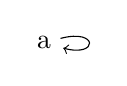
\begin{tikzpicture}[baseline=(a.base)]
\node (a) {a};
\draw (a) edge[loop right] (a);
\end{tikzpicture}

\begin{itemize}
    \item Terminating? No
    \item Confluent? Yes
    \item Unique normal forms? No, because a looping final element can't really be final. 
\end{itemize}

\subparagraph{ARS 4}
\[
A = \{a,b,c\}, \quad R = \{(a,b),(a,c)\}
\]

\textbf{Picture:}
\begin{tikzpicture}[baseline=(a.base)]
\node (a) {a};
\node (b) [below left of=a] {b};
\node (c) [below right of=a] {c};
\draw (a) -> (b);
\draw (a) -> (c);
\end{tikzpicture}

\begin{itemize}
    \item Terminating? Yes
    \item Confluent? No, $a$ leads to two different elements which don't converge
    \item Unique normal forms? No, as the elements don't converge back to the same final element.
\end{itemize}

\subparagraph{ARS 5}
\[
A = \{a,b\}, \quad R = \{(a,a),(a,b)\}
\]

\textbf{Picture:}
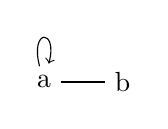
\begin{tikzpicture}[baseline=(a.base)]
\node (a) {a};
\node (b) [right of=a] {b};
\draw (a) edge[loop above] (a);
\draw (a) -> (b);
\end{tikzpicture}

\begin{itemize}
    \item Terminating? No, $a$ can be looped upon indefinitely.
    \item Confluent? Yes, because $a$ has to end at $b$ if ends at all.
    \item Unique normal forms? Yes
\end{itemize}

\subparagraph{ARS 6}
\[
A = \{a,b,c\}, \quad R = \{(a,b),(b,b),(a,c)\}
\]

\textbf{Picture:}
\begin{tikzpicture}[baseline=(a.base)]
\node (a) {a};
\node (b) [below left of=a] {b};
\node (c) [below right of=a] {c};
\draw (a) -> (b);
\draw (a) -> (c);
\draw (b) edge[loop left] (b);
\end{tikzpicture}

\begin{itemize}
    \item Terminating? No, has a loop.
    \item Confluent? No
    \item Unique normal forms? No, loop makes $b$ irreducible 
\end{itemize}

\subparagraph{ARS 7}
\[
A = \{a,b,c\}, \quad R = \{(a,b),(b,b),(a,c),(c,c)\}
\]

\textbf{Picture:}
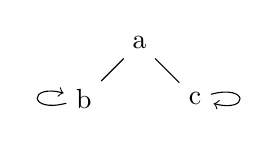
\begin{tikzpicture}[baseline=(a.base)]
\node (a) {a};
\node (b) [below left of=a] {b};
\node (c) [below right of=a] {c};
\draw (a) -> (b);
\draw (a) -> (c);
\draw (b) edge[loop left] (b);
\draw (c) edge[loop right] (c);
\end{tikzpicture}

\begin{itemize}
    \item Terminating? No, has loops.
    \item Confluent? No
    \item Unique normal forms? No, loops make $b$ and $c$ irreducible
\end{itemize}

\paragraph{Part 2}

Find an example of an ARS for each of the possible 8 combinations.

Format: True or false (T or F) for (Confluent, Terminates, UNF)

\begin{enumerate}
    \item \textbf{(T, T, T)} 
    Example: ARS \#2

    \item \textbf{(T, T, F)} 
    Example: impossible. \\
    Reason: if ARS is fully reducible and terminates, there must be multiple elements that converge into one element. Therefore, this ARS won't have more than 1 normal form, despite 3 elements, hence it doesn’t have unique normal forms.

    \item \textbf{(T, F, T)} 
    Example: ARS \#5

    \item \textbf{(T, F, F)} 
    Example: ARS \#3

    \item \textbf{(F, T, T)} 
    Example: impossible. 
    Reason: ARS is terminating and has unique normal forms, which implies confluence towards one element, which 
    is supposed to be false, so impossible.

    \item \textbf{(F, T, F)} 
    Example: ARS \#4

    \item \textbf{(F, F, T)} 
    Example: impossible. 
    Reason: If an ARS has unique normal forms, then it implies multiple elements confluencing to one element, which is
    false here, so impossible.

    \item \textbf{(F, F, F)} 
    Example: ARS \#6, ARS \#7
\end{enumerate}

\subsubsection{Questions}

HW 2 Question: So it seems like an ARS with unique normal forms should always reach the last element unless there's a non-terminating relation somewhere in the ARS. 
Is this true? if so, are there other uses for tracking terminability in ARS's?

\section{Essay}

\section{Evidence of Participation}

\section{Conclusion}\label{conclusion}

\begin{thebibliography}{99}
\bibitem[BLA]{bla} Author, \href{https://en.wikipedia.org/wiki/LaTeX}{Title}, Publisher, Year.
\end{thebibliography}

\end{document}
